\documentclass[xcolor=pdftex,dvipsnames]{beamer}

\usepackage{amsmath}
\usepackage{amssymb}

\usepackage{comment}
\usepackage{textcomp}

\title{Microeconomic Theory --- ECON 323 503 \\ Chapter 9: Properties
  and applications of the competitive model}
\author{Vikram Manjunath}       %
\institute{Texas A\&M University}
\setbeamertemplate{navigation symbols}{}
\setbeamertemplate{footline}{}
\usefonttheme{serif}
\begin{document}

\maketitle

\begin{frame}
\frametitle{Outline}
\begin{enumerate}[<+->]
\item Zero-profit for competitive firms in the long run: This happens
  even when entry is limited.
\item Producer surplus: a measure of firms' gains and losses when
  there is a change in the equilibrium.
\item Competition maximizes welfare: welfare, the sum of consumer and
  producer surpluses, is maximal in equilibrium.
\item Policies that shift the supply curve: limiting entry and exit.
\item Policies that create a wedge between supply and demand curves:
  taxes, price ceilings, price floors, and tariffs.
\end{enumerate}
\end{frame}




\begin{frame}
\frametitle{Zero profit for competitive firms in the long run}
Zero (\emph{economic}) profit.

\bigskip
\uncover<2->{Previous chapter: zero profit when entry is unrestricted.}
\bigskip

\uncover<3->{What if entry is limited?}
\bigskip

\uncover<4->{Example: land. There's only so much of it.}
\end{frame}



\begin{frame}
\frametitle{Zero profit for competitive firms in the long run}
\begin{center}
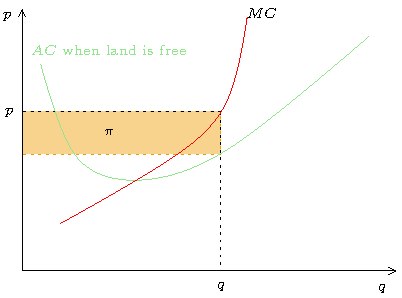
\includegraphics{pics/ZeroProfitLand}
\end{center}
Land use is free: profit is $\pi=pq-C(q) = pq-qAC(q)$.
\end{frame}



\begin{frame}
\frametitle{Zero profit for competitive firms in the long run}
What if there are many farmers who would like to use the land?
\bigskip

\uncover<2->{How much rent should the landowner charge?}
\bigskip

\uncover<3->{Answer: $\pi$}
\bigskip

\uncover<4->{That's the opportunity cost of renting out the land. His alternative
is to farm the land himself.}
\bigskip

\uncover<5->{Rent paid for the land is a fixed (avoidable) cost. It doesn't change
with $q$.}
\bigskip

\uncover<6->{$AC$ curve shifts up.}
\end{frame}



\begin{frame}
\frametitle{Zero profit for competitive firms in the long run}
\begin{center}
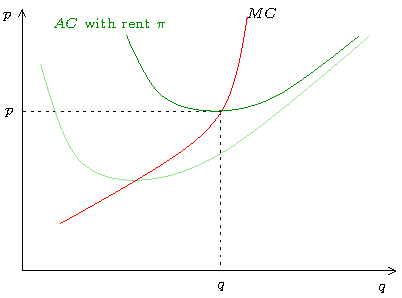
\includegraphics{pics/ZeroProfitLandA}
\end{center}
If rent is $\pi$, profit (after paying rent) is zero.
\end{frame}



\begin{frame}
\frametitle{An implication of zero profit }
The highest long run profit is zero.
\bigskip

\uncover<2->{Any firm that is not maximizing profit makes a lower profit than zero.}
\bigskip

\uncover<3->{In other words: if you're not maximizing profit, you're losing money.}
\bigskip

\uncover<4->{So firms that do not maximize profit go out of business in the long run.}

\end{frame}



\begin{frame}
\frametitle{Producer surplus}
\emph{Producer surplus:} the firm's gain from participating in the
market.

\bigskip
\uncover<2->{$=$ What you earn selling $q - \text{minimum}$  you need to supply $q$.}

\bigskip
\uncover<3->{Analog of consumer surplus.}

 
\end{frame}



\begin{frame}
\frametitle{Producer surplus}
\begin{center}
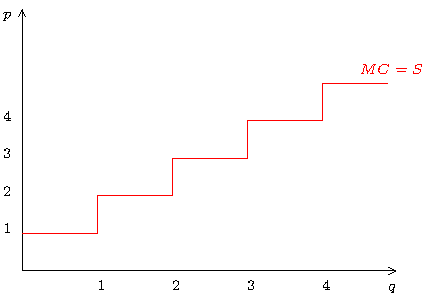
\includegraphics{pics/PS1}
\end{center}
$MC$/supply curve tells us how much it costs the firm to produce the
first unit, the second unit, and so on.
\end{frame}

\begin{frame}
\frametitle{Producer surplus}
\begin{center}
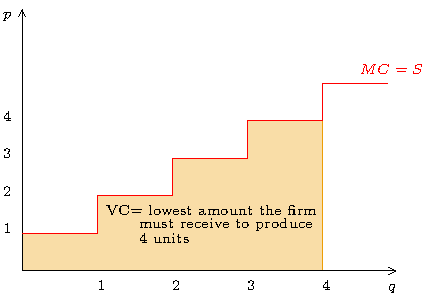
\includegraphics{pics/PS2}
\end{center}
From this we learn minimum amount that the firm needs to produce $q$
units of the good. This is just $VC(q)$.
\end{frame}

\begin{frame}
\frametitle{Producer surplus}
\begin{center}
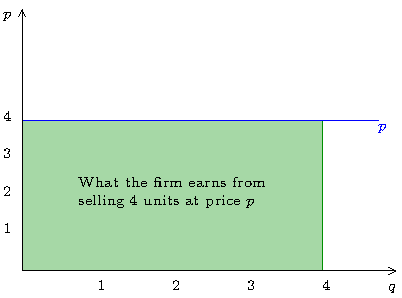
\includegraphics{pics/PS3}
\end{center}
If the price is $p$, the firm earns $pq$ from selling $q$ units of the good.
\end{frame}

\begin{frame}
\frametitle{Producer surplus}
\begin{center}
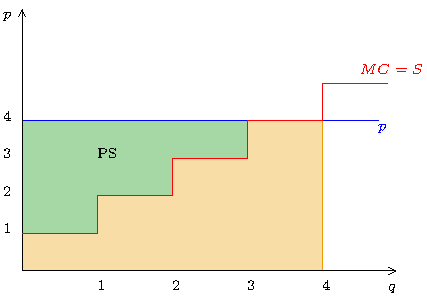
\includegraphics{pics/PS4}
\end{center}
PS $=$ What you earn selling $q - \text{minimum}$  you need to supply $q$.
\\
\
\end{frame}



\begin{frame}
\frametitle{Producer surplus}
\begin{center}
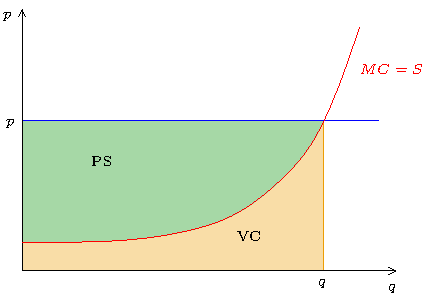
\includegraphics{pics/PS5}
\end{center}
In general, PS is the area \emph{above} the
supply curve and below the line at the price.

\end{frame}



\begin{frame}
\frametitle{Producer surplus vs profit}
Area below the supply curve is VC.
\bigskip

\uncover<2->{
Why? Because it's the integral of the marginal cost!
}\bigskip

\uncover<3->{Area below line at the price is $pq = R$.}
\bigskip

\uncover<4->{So \[
PS = R-VC.
\]}



\uncover<5->{Remember that 
\[
\pi = R- C = R- VC - F.
\]}

\uncover<6->{
So 
\[
PS - \pi = F.
\]}
\uncover<7->{The difference between PS and profit is just fixed cost.}

\end{frame}



\begin{frame}
\frametitle{Measuring society's welfare}
One possible measure of society's wellbeing:
\[
W = PS + CS.
\]

\uncover<2->{$W$ is the total gains from the market being allowed to operate: the
producers' gains(PS) and the consumers' gains (CS).}


\uncover<3->{\bigskip
Note: This is one particular way of measuring welfare. It's weights
everyone (producer and consumer) equally and adds up their
welfare. It's as though welfare of two different actors are
\emph{perfect substitutes.}}

\end{frame}

\begin{frame}
\frametitle{Graphically}
\begin{center}
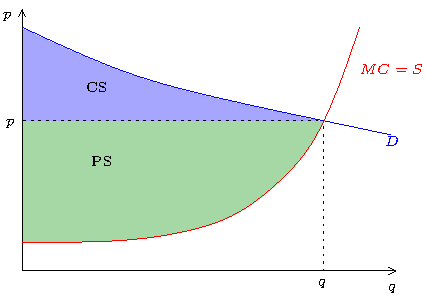
\includegraphics{pics/W}
\end{center}
Total welfare, the sum of consumer and producer surpluses is the area
above the supply curve and below the demand curve.
\end{frame}

\begin{frame}
\frametitle{Producing less than the  competitive output reduces $W$}
\begin{center}
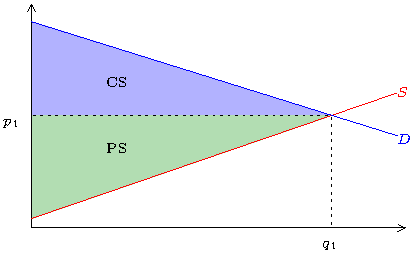
\includegraphics{pics/CEEff1}
\end{center}
Start with the equilibrium price and quantity.
\end{frame}
\begin{frame}
\frametitle{Producing less than the  competitive output reduces $W$}
\begin{center}
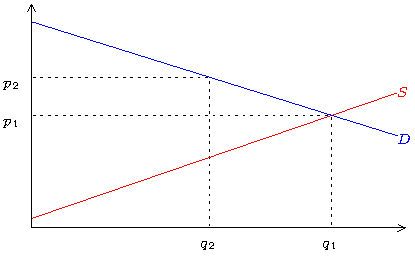
\includegraphics{pics/CEEff2}
\end{center}
Suppose that quantity falls to $q_2$ and price rises to $p_2$.
\end{frame}
\begin{frame}
\frametitle{Producing less than the  competitive output reduces $W$}
\begin{center}
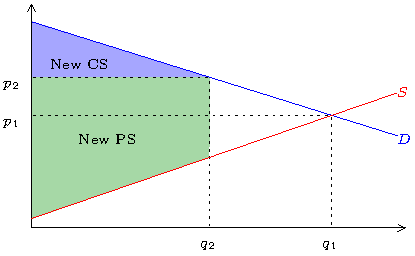
\includegraphics{pics/CEEff3}
\end{center}
PS and CS change.\end{frame}

\begin{frame}
\frametitle{Producing less than the  competitive output reduces $W$}
\begin{center}
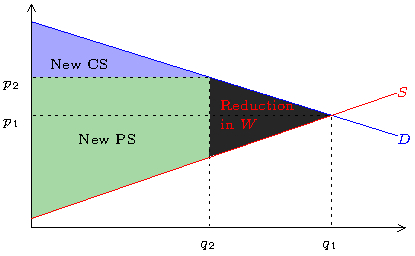
\includegraphics{pics/CEEff4}
\end{center}
There is a loss of welfare when this happens.
\end{frame}



\begin{frame}
\frametitle{Deadweight loss}
\begin{center}
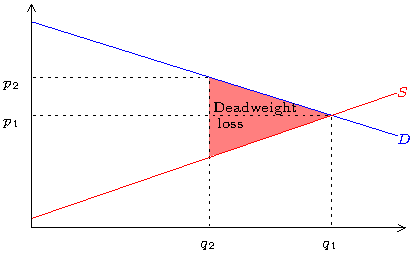
\includegraphics{pics/DWL}
\end{center}
\emph{Deadweight loss}: The loss of surplus by one group that is not
offset by a gain to another group.
\end{frame}



\begin{frame}
\frametitle{Producing more than the competitive output reduces $W$}
\begin{center}
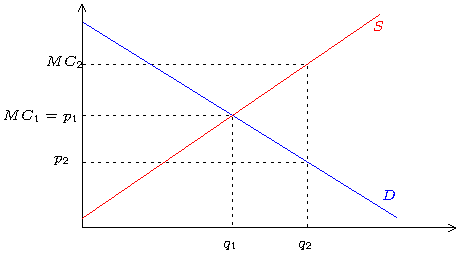
\includegraphics{pics/CEEff5}
\end{center}
Start with $q_1$ at price $p_1$ and think about what happens when we
move to $q_2$ at $p_2$.
\end{frame}

\begin{frame}
\frametitle{Producing more than the competitive output reduces $W$}
\begin{center}
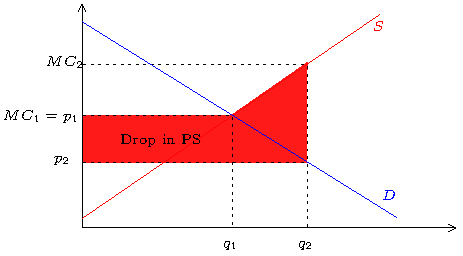
\includegraphics{pics/CEEff6}
\end{center}
Firms receive a lower price ($p_2<p_1$) \emph{and} their marginal cost
rises. So there's a loss of PS.
\end{frame}

\begin{frame}
\frametitle{Producing more than the competitive output reduces $W$}
\begin{center}
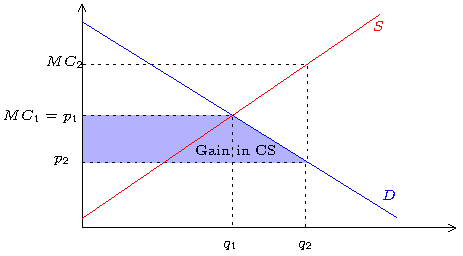
\includegraphics{pics/CEEff7}
\end{center}
Consumers pay less and consume more. So there's a gain in CS.\\
\
\end{frame}
\begin{frame}
\frametitle{Producing more than the competitive output reduces $W$}
\begin{center}
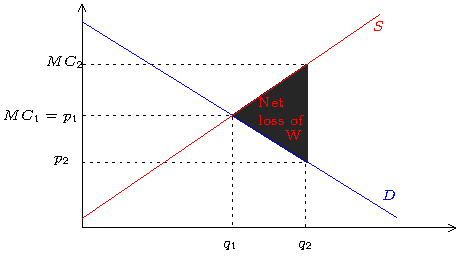
\includegraphics{pics/CEEff8}
\end{center}
The firms' loss isn't entirely offset by the consumers' gain. So
overproducing leads to a deadweight loss too.
\end{frame}



\begin{frame}
\frametitle{Policies that shift the supply curve}
Two simple ways of doing this:
\begin{enumerate}
[<+->]
\item Entry barriers: if firms cannot enter freely, the market supply
  curve shifts to the left.
\item Exit restrictions: short-run number of firms would be high. In
  the long run, fewer firms would enter the market.

\end{enumerate}
\end{frame}



\begin{frame}
\frametitle{Policies that create a wedge between $S$ and $D$}
We'll consider two kinds of policies:
\begin{enumerate}[<+->]
\item Sales tax: specific tax on the good. Government raises revenue
  of $T$. So $W=PS+CS+T$.
\item Price floor: guarantee that the price won't be below $\underline
  p$. Government spends $X$ to keep price at $\underline p$. So $W=PS+CS-X$.
\end{enumerate}
\bigskip
\end{frame}



\begin{frame}
\frametitle{Sales tax}
\begin{center}
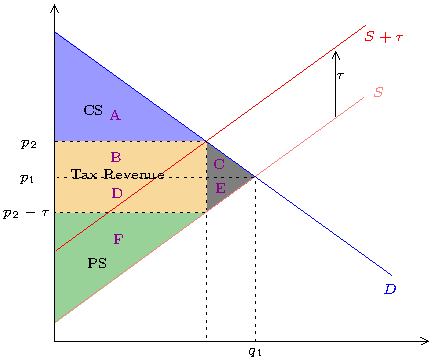
\includegraphics{pics/EffectOfSalesTax}

\begin{tabular}{|c|c|c|}\hline &Without tax & With tax\\
\hline CS & A+B+C & A\\
\hline PS & D+E+F & F\\
\hline Tax revenue & 0 & B+D
\\
\hline
\end{tabular}
\end{center}
\end{frame}


\begin{frame}
\frametitle{Price floor}
\begin{center}
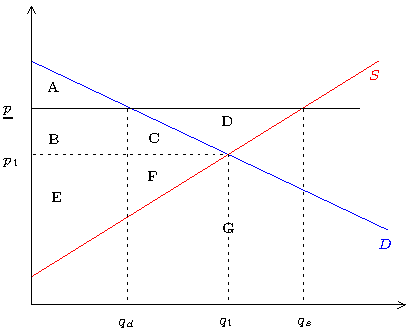
\includegraphics{pics/PriceFloor}
\end{center}
\vspace{0.8in}
\end{frame}

\begin{frame}
\frametitle{Price floor}
\begin{center}
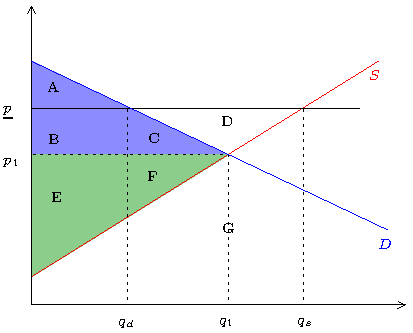
\includegraphics{pics/PriceFloorA}

\begin{tabular}{|c|c|c|}\hline &Without tax & With tax\\
\hline CS & A+B+C & \\
\hline PS & E+F &  {\color{white}B+C+D+E+F}\\
\hline Government expense& 0 & {\color{white}C+D+E+F}
\\
\hline
\end{tabular}
\end{center}
\end{frame}




\begin{frame}
\frametitle{Price floor}
\begin{center}
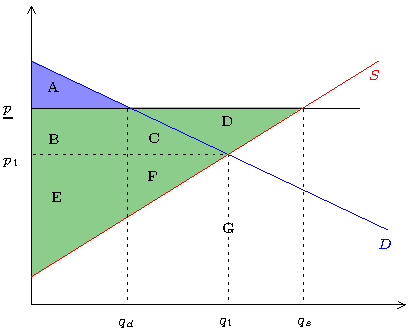
\includegraphics{pics/PriceFloorB}

\begin{tabular}{|c|c|c|}\hline &Without tax & With tax\\
\hline CS &A+B+C& A \\
\hline PS & E+F& B+C+D+E+F \\
\hline Government expense& 0 & 
\\
\hline
\end{tabular}
\end{center}
\end{frame}

\begin{frame}
\frametitle{Price floor}
\begin{center}
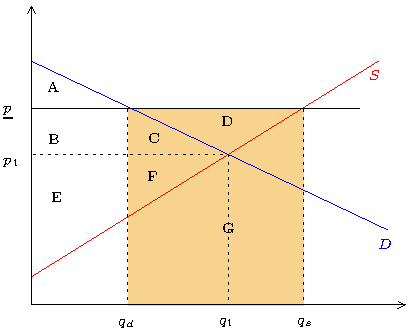
\includegraphics{pics/PriceFloorC}

\begin{tabular}{|c|c|c|}\hline &Without price floor & With price floor\\
\hline CS &A+B+C& A \\
\hline PS & E+F& B+C+D+E+F \\
\hline Government expense, $X$& 0 & C+D+F+G
\\
\hline
\end{tabular}
\end{center}
\end{frame}

\begin{frame}
\frametitle{Price floor}
\begin{center}
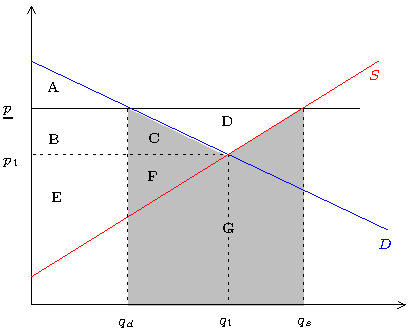
\includegraphics{pics/PriceFloorD}

\begin{tabular}{|c|c|}
\hline&Total welfare, $W=CS+PS-X$\\\hline
With price floor& A+B+C+E+F\\\hline
Without price floor& A+B+E-G\\\hline
\end{tabular}
\medskip

Total welfare
Deadweight loss is C+F+G.
\end{center}
\end{frame}





\begin{frame}
\frametitle{Rent seeking}
Many policies carry a deadweight loss (a reduction in $W$). 
\bigskip

\uncover<2->{
But we see them all the time.
\bigskip
}

\uncover<3->{ Though $W$ drops: one of $PS$ or $CS$ rises while the other falls.
}

\bigskip
\uncover<4->{ The increase in one isn't enough to offset the decrease in the other.}
\bigskip

\uncover<5->{ The ``winner'' in the situation has an incentive to persuade (lobby,
influence, bribe) a government to enact such policies.}
\bigskip

\uncover<6->{ This is \emph{rent seeking} behavior.}
\end{frame}

\end{document}







